% kapitel2.tex
\chapter{Implemented Changes}
\label{chapter:implementedChanges}

This work extends Tour4Me\footnote{\url{http://tour4me.cs.tu-dortmund.de/}}, which is an application written in C++ and HTML. 
The implemented interface uses C\# as programming language to enable easy porting of the web application to a desktop or mobile application.
To improve the query times, a spatial database was added. 
Reasons for and positive effects of this decision are described in the following section.

Furthermore, not only the language and data access was changed.
New options and parameters to improve the customizability of preferences for a generated tour were added as well.
These changes had to be incorporated into an upgraded front end design (see sections \ref{subsec:interfaceAndFrontendChanges} and \ref{sec:parameterChanges}) as well as into the back end and all solvers (see section \ref{sec:algorithmicChanges}). 


\section{Application}
\label{sec:application}

To include the various changes, the whole application was changed.
The Open Street Map (OSM) data are downloaded and stored in a database.
The graph for calculating the roundtrips is thus build from the new database.
Furthermore, the whole design of the front end was changed to improve the overview and general user experience as well as to allow for the addition of new customization options.
Lastly, the algorithms to choose from have been extended by two additional meta-heuristic approaches.

\subsection{New Architecture}
\label{sec:newArchitecture}

For the new application, the architecture had to be re-structured.
An illustration of the new design is shown in figure \ref{fig:architecture}.
Instead of reading the data for the graph from a static .txt file, which contains all the nodes and edges for Dortmund, a database is used to manage the nodes, edges, their additional information and the relationships between them. 
It can be filled with the data needed by using an import python script that creates an osmnx-graph\footnote{\url{https://osmnx.readthedocs.io/en/stable/}, last accessed: 15.04.2024}\footnote{\url{https://networkx.org/}, last accessed: 22.03.2024}\footnote{\url{https://wiki.openstreetmap.org}, last accessed: 22.03.2024}\footnote{\url{https://wiki.openstreetmap.org/wiki/Main_Page}, last accessed: 19.04.2024} add all references for a user specified location. 
From this graph, the nodes and edges can be extracted alongside their additional information.
For the current use case, nodes are stored with their OSM-ID, which is transformed into a UUID, their latitude and longitude coordinates as well as their elevation profile and tags of the surroundings they are placed in.
The elevation data has to be acquired from a different source than OSM, since they do not use a height profile. 
A few open source providers were available, but ultimately, Open-Elevation\footnote{\url{https://open-elevation.com/}, last accessed: 20.03.2024} was used. 

Since most open source providers have a limited bandwidth to supply users with data based on their API-calls, the opportunity to use a locally hosted version that Open-Elevation offered was very important to assure usability.
When using the python script to create and fill the database and its tables, the Open-Elevation data needs to be available.
A local docker container with the respective data can be used to access the needed information without being bound to the servers and their throughput boundaries.

The used database is Microsoft SQL Server Management Studio\footnote{\url{https://learn.microsoft.com/en-us/sql/sql-server/sql-docs-navigation-guide?view=sql-server-ver16}, last accessed: 22.03.2024}, which can handle spatial data, supports spatial queries and works well in combination with the C\# implementation.

The back end is written in C\#\footnote{\url{https://learn.microsoft.com/en-us/dotnet/csharp/}, last accessed: 22.03.2024}, as this language allows for the opportunity to also create a mobile- or desktop application in addition to the web application that already exists (see \ref{sec:futureWork}).
Furthermore, C\# allows for using SQL queries and filtering using LINQ for easy runtime database querying\footnote{\url{https://docs.telerik.com/devtools/aspnet-ajax/controls/grid/asp.net-3.5-features/linq-to-sql---binding-and-automatic-crud-operations}, last accessed: 22.03.2024}.


The front end is implemented using HTML\footnote{\url{https://devdocs.io/html/}, last accessed: 22.03.2024}, CSS\footnote{\url{https://devdocs.io/css/}, last accessed: 22.03.2024}, JavaScript\footnote{\url{https://devdocs.io/javascript/}, last accessed: 22.03.2024} and C\# code behind. 
Here, the base-styling is done using bootstrap\footnote{\url{https://getbootstrap.com/docs/4.3/getting-started/introduction/}, last accessed: 22.03.2024}, but additional custom CSS is added to create a nature-based color palette (\#TODO references to color theory stuff?) as well as several effects for the side and bottom menus.
To realize the communication between front end and back end, Ajax-queries\footnote{\url{https://api.jquery.com/category/ajax/}. last accessed: 22.03.2024} are used.

The map is a leaflet\footnote{\url{https://leafletjs.com/}, last accessed: 20.03.2024} visualization that shows Open Street Map data.
The leaflet map allows to set markers, add a search bar, create polygons - which are used to illustrate the generated routes - and offers an open source map view. 


\begin{figure}[ht]
	\hspace*{-25 pt}
	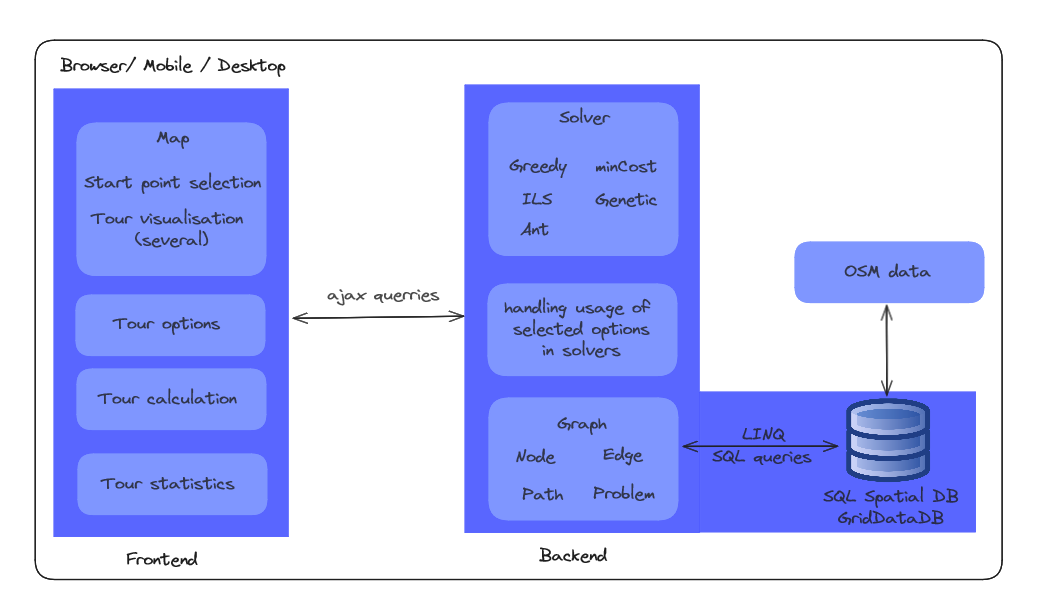
\includegraphics[width=1.1\textwidth]{bilder/Implementation Architecture.png}
	\caption{Visualization of the used architecture}
	\label{fig:architecture}
\end{figure}


In the above visualization, the whole application, the distinct parts and features are illustrated. 
The front end is realized as a web application, running in the browser but can also be customized to be executable as a mobile or desktop application (see \ref{sec:futureWork}).
Here, the map is visualized using leaflet. 
In this map, the marker can be set to the current location - if the permission to access the data is granted.
However simply searching for a specific address, drag-and-dropping the marker on the map, or scrolling the map and selecting a position by clicking on the place to mark are also possible. 
Furthermore, the visualization of the calculated tours is also realized using the map and a polygon built from the respective points.
For debug purposes, there is a feature to show the whole graph that is being used for the calculation using the current maximum length.

In addition to the main feature - the map - the front end also contains two menus:
One holding the parameters the user can use to customize the tours according to their preferences and the information menu containing a report of the core data of the calculated path that is being visualized. 
A more detailed description of the front end design, concept sketches and the final implementation are outlined in subsection \ref{subsec:interfaceAndFrontendChanges}.

\subsection{Database}
\label{subsection:database}

The database is a relational database using Microsoft SQL server, administered in Microsoft SQL Server Management Studio.
This database also allows to use spatial data, which was an important feature for storing and processing the nodes and edges.
Using the spatial features enables the possibilities to filter nodes within a given radius, retrieving only a relevant subset of data points.
This filtering option within the database significantly speeds up the data retrieval as well as the graph creation.
Compared to the previous method of generating a fixed graph for the city of Dortmund, the database offers further important advantages:
Far more nodes than only points within Dortmund can be used.
Despite the database creation and the adding of points being relatively slow, this is a process that only needs to be ran once and does not affect the tour calculation. 
Once the data has been added, all points can be accessed without needing to retrieve the whole database.

To create the database, a python script is used. \# TODO if added, describe parameters and how to use the script with them
This script first creates an osmnx graph from OSM data using the \texttt{graph\textunderscore from\textunderscore place} function
\begin{lstlisting}
	ox.graph_from_place(place_name, network_type='all', custom_filter=custom_filter)
\end{lstlisting}

Here, the \texttt{place\textunderscore name} is the name of the place for which osmnx data should be gathered.
For a city, the city's name, state and country need to be added. 
If a whole state should be selected, the state name and country are required.
The network\textunderscore type has six values to choose from\footnote{\url{https://osmnx.readthedocs.io/en/stable/user-reference.html\#module-osmnx.settings}, last accessed: 19.04.2024}: "all\textunderscore private", "all", "bike", "drive", "drive\textunderscore service", and "walk". 

The \texttt{custom\textunderscore filter} is defined to select only those edges, where walking, running and cycling is possible by specifically de-selecting respective highway types:

\begin{lstlisting}
	custom_filter = '["highway"]["highway"!~"motorway|trunk|proposed|construction|motorway_link|trunk_link"]'
\end{lstlisting}

The excluded types are used for the following street types according to the OSM Wiki:


Next, the elevation data has to be added for the nodes of this graph.
These information are not part of osmnx but need to be retrieved from a different source.
For this thesis, Open Elevation\footnote{\url{https://open-elevation.com/}, last accessed: 20.03.2024} was used.


\begin{table}[ht]
	\centering
	\begin{tabular}{l|l}
		Highway type & Description\\
		\hline
		motorway & A restricted access major divided highway, normally with 2\\ 
		& or more running lanes plus emergency hard shoulder.\\
		& Equivalent to the Freeway, Autobahn, etc..  \\
		trunk & The most important roads in a country's system that aren't \\
		& motorways. (Need not necessarily be a divided highway.) \\
		proposed & For planned roads. \\
		construction & For roads under construction. \\
		motorway\textunderscore link & The link roads (sliproads/ramps) leading\\
		& to/from a motorway from/to a motorway or lower class highway. \\
		& Normally with the same motorway restrictions. \\
		trunk\textunderscore link & The link roads (sliproads/ramps) leading \\
		& to/from a trunk road from/to a trunk road or lower class highway. 
	\end{tabular}
	\caption[OSM highway types]{This table shows a listing of different OSM highway types and their definition taken from the Wiki page\protect\footnotemark}
	\label{tab:osmHighwayTypes}
\end{table}

\footnotetext{\url{https://wiki.openstreetmap.org/wiki/Key:highway}, last accessed: 19.04.2024}
The 


\subsection{Interface and Front end changes}
\label{subsec:interfaceAndFrontendChanges}

\begin{figure}[H]
	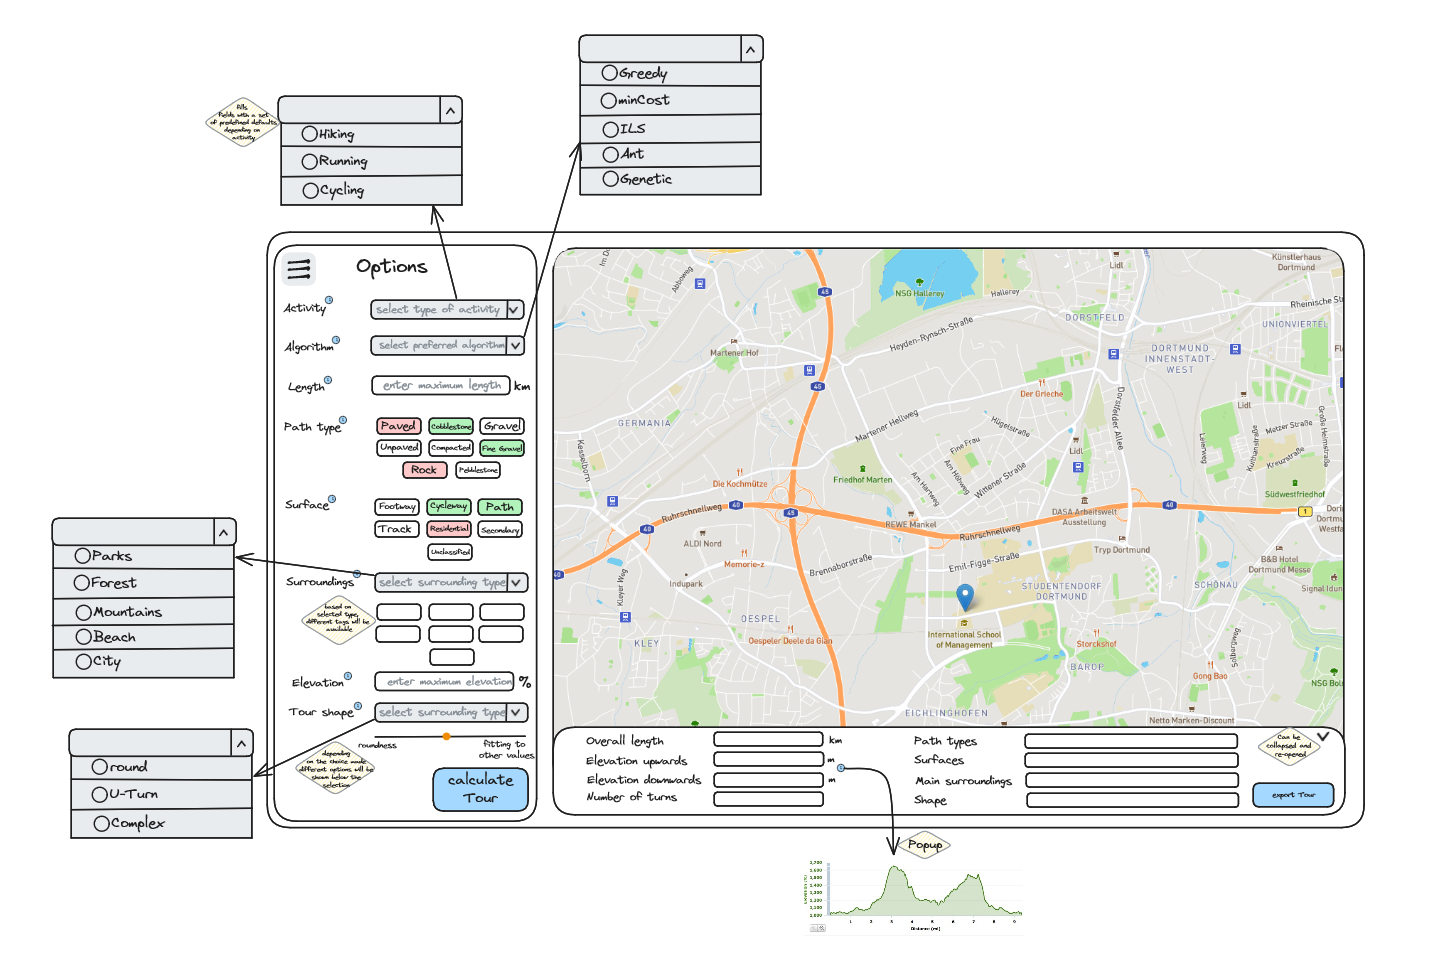
\includegraphics[width=0.9\linewidth]{bilder/Concept new Frontend design.png}
	\caption{Design concept for the front end view, including descriptions for drop-downs and pop-ups}
	\label{fig:frontendConcept}
\end{figure}


\begin{figure}[H]
	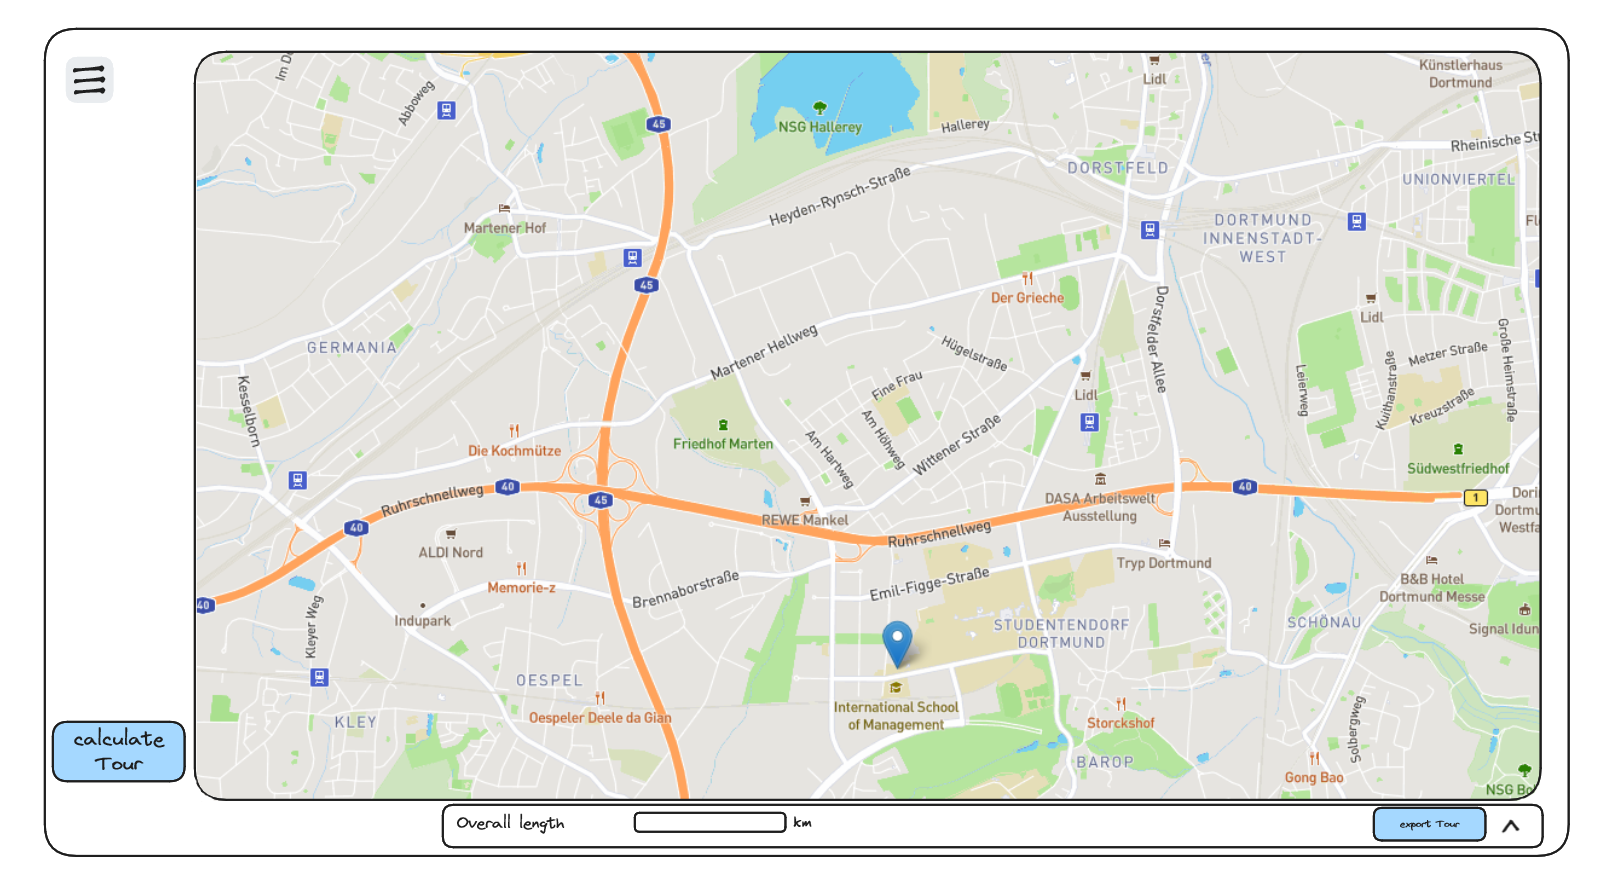
\includegraphics[width=0.9\linewidth]{bilder/Concept burger menu and stats hidden.png}
	\caption{Design concept for the front end view with all menus folded}
	\label{fig:frontendConceptMenusClosed}
\end{figure}


\begin{figure}[H]
	\begin{subfigure}[t]{0.9\linewidth}
		\centering
		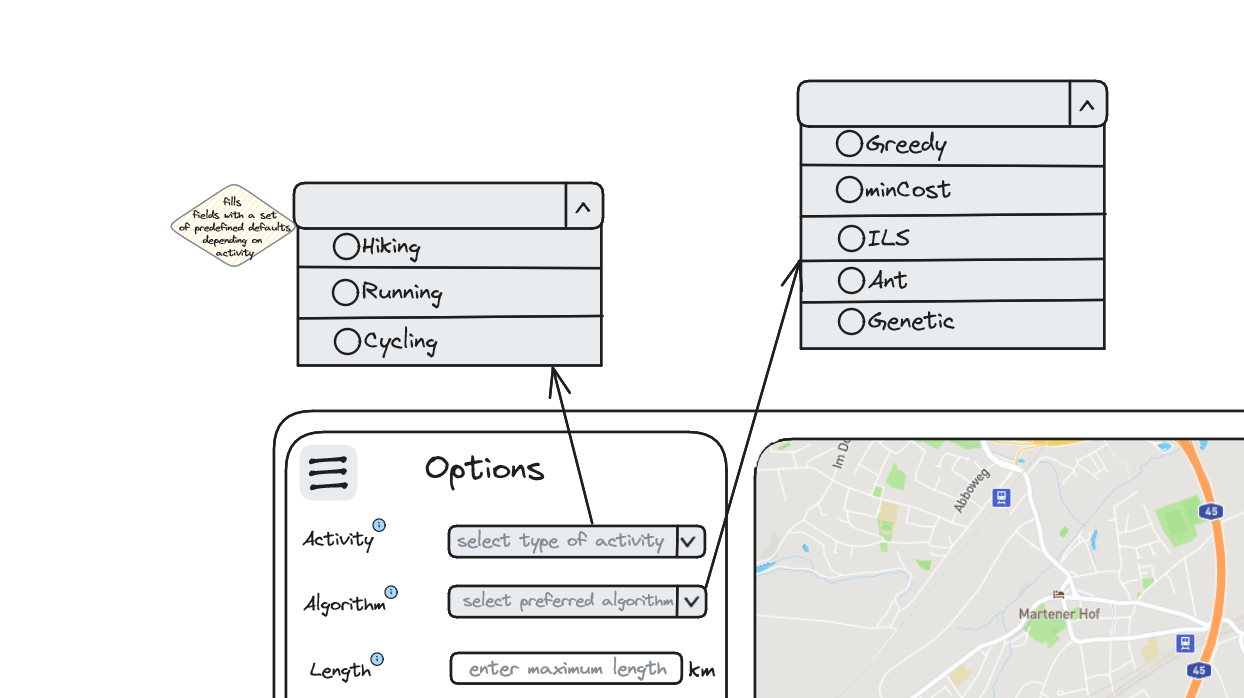
\includegraphics[width=\linewidth]{bilder/Concept closeup activity, algorithm.png}
		\caption{Design concept for the front end view, closeup of activity and algorithm dropdowns}
		\label{fig:frontendConceptCloseupDropdowns}	
	\end{subfigure}
	\hfill
	\begin{subfigure}[t]{0.9\linewidth}
		\centering
		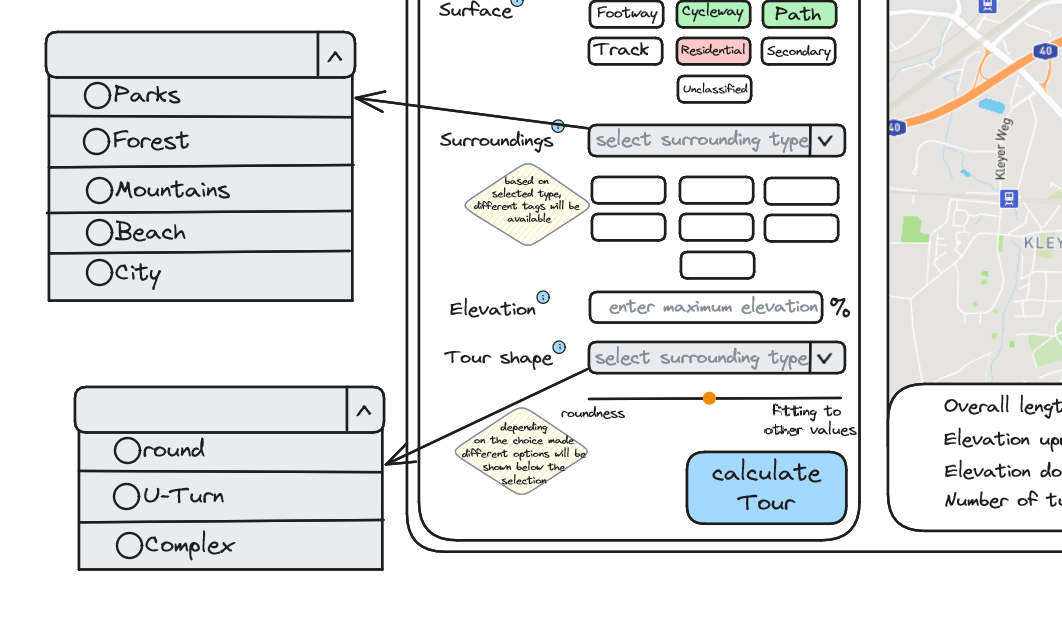
\includegraphics[width=\linewidth]{bilder/Concept closeup surroundings, tour shape.png}
		\caption{Design concept for the front end view, closeup of a surrounding and Tour shape}
		\label{fig:frontendConceptCloseupButtons}		
	\end{subfigure}
\end{figure}


\begin{figure}[H]
	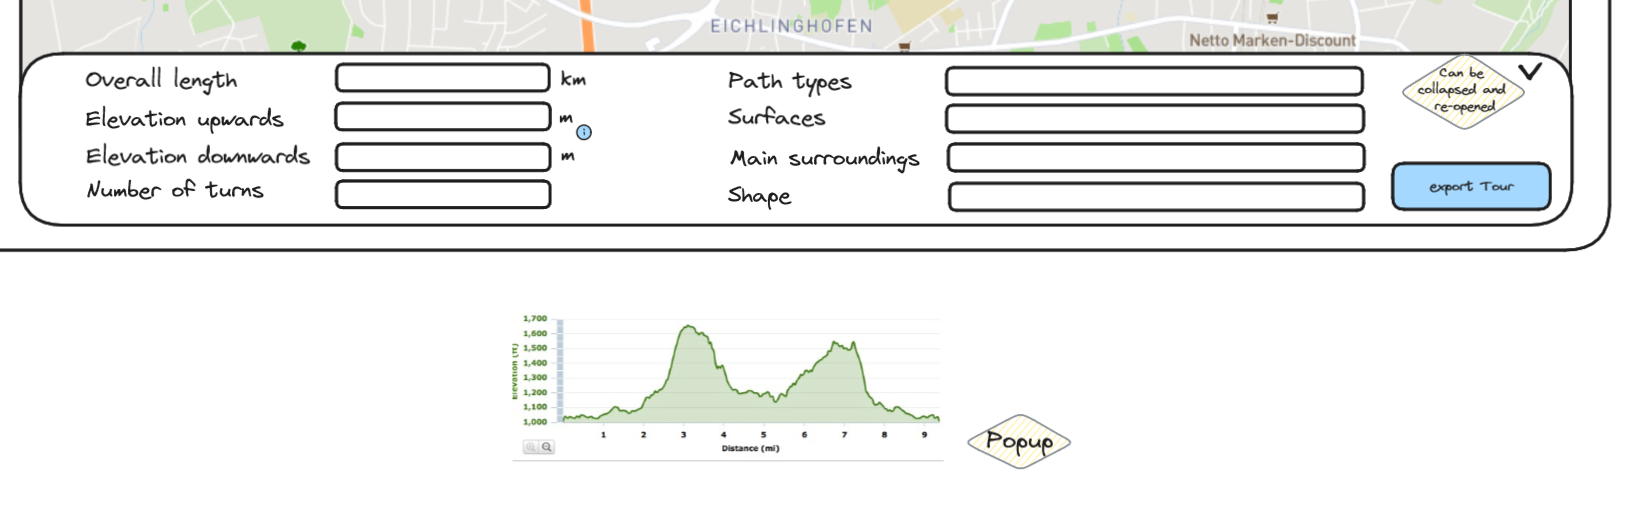
\includegraphics[width=0.9\linewidth]{bilder/Concept closeup tour stats, elevation profile.png}
	\caption{Design concept for the front end view, closeup of the results view}
	\label{fig:frontendConceptResultsCloseup}
\end{figure}



\section{Algorithmic changes}
\label{sec:algorithmicChanges}

\subsection{Ant Colony}
\label{subsec:antColonyImplementation}

\subsection{Genetic Algorithms}
\label{subsec:geneticAlgorithmsImplementation}

\subsection{Simulated Annealing}
\label{subsec:simulatedAnnealingImplementation}

\section{Parameter changes}
\label{sec:parameterChanges}

